\documentclass{beamer}

%Packages
\usepackage[utf8]{inputenc}
\usepackage{hyperref}
\usepackage{setspace}

\usepackage{listings}
\usepackage{xcolor}

\definecolor{lightgrey}{rgb}{0.92,0.92,0.92} % defining color for listing
\definecolor{darkgreen}{rgb}{0,0.6,0} % defining color for listing
\colorlet{punct}{red!60!black}
\definecolor{background}{HTML}{EEEEEE}
\definecolor{delim}{RGB}{20,105,176}
\colorlet{numb}{magenta!60!black}

\lstdefinelanguage{JavaScript}{
  keywords={typeof, new, true, false, catch, function, return, null, catch, switch, var, if, in, while, do, else, case, break},
  keywordstyle=\color{blue}\bfseries,
  ndkeywords={class, export, boolean, throw, implements, import, this},
  ndkeywordstyle=\color{darkgray}\bfseries,
  identifierstyle=\color{black},
  sensitive=false,
  comment=[l]{//},
  morecomment=[s]{/*}{*/},
  commentstyle=\color{purple}\ttfamily,
  stringstyle=\color{red}\ttfamily,
  morestring=[b]',
  morestring=[b]"
}
\lstset{language=JavaScript,
  basicstyle=\tiny\ttfamily,
  stepnumber=1,
  numbersep=8pt,
  showstringspaces=false,
  breaklines=true,
  backgroundcolor=\color{lightgrey},
  literate=
   *{0}{{{\color{numb}0}}}{1}
    {1}{{{\color{numb}1}}}{1}
    {2}{{{\color{numb}2}}}{1}
    {3}{{{\color{numb}3}}}{1}
    {4}{{{\color{numb}4}}}{1}
    {5}{{{\color{numb}5}}}{1}
    {6}{{{\color{numb}6}}}{1}
    {7}{{{\color{numb}7}}}{1}
    {8}{{{\color{numb}8}}}{1}
    {9}{{{\color{numb}9}}}{1}
    {:}{{{\color{punct}{:}}}}{1}
    {,}{{{\color{punct}{,}}}}{1}
    {\{}{{{\color{delim}{\{}}}}{1}
    {\}}{{{\color{delim}{\}}}}}{1}
    {[}{{{\color{delim}{[}}}}{1}
    {]}{{{\color{delim}{]}}}}{1},
}

% Hide navigation symbols, show git
\setbeamertemplate{navigation symbols}{}
\setbeamertemplate{footline}[frame number]

\newcommand{\inote}[1]{
  {
    \begin{itemize}
      \item #1
    \end{itemize}
  }
}

% Logos
\newcommand{\logoimage}[2]{\begingroup
\setbox0=\hbox{\includegraphics[height=#2]{#1}}%
\parbox{\wd0}{\box0}\endgroup\ }

%META-INFORMATION
\title{\logoimage{imgs/logo}{40px}\\A document-oriented database}
\author{Tom Wiesing}
\institute{Databases \& Web Applications}
\date{November 2, 2015}

\begin{document}
    %TITLEPAGE
    \frame{\titlepage}

    \begin{frame}{Overview}
      \begin{itemize}
          \item Introduction \& Structure of MongoDB
          \item CRUD operations \& Basic querying
          \item Aggregation Operations
          \item Advanced Write Operations
          \item Summary \& Further topics
      \end{itemize}
    \end{frame}

    \begin{frame}{Introduction (1): What are document-oriented databases?}
  \begin{columns}[onlytextwidth]
    \begin{column}{0.6\textwidth}
      \begin{itemize}
          \item stuff
            \inote{...}
      \end{itemize}
    \end{column}
    \begin{column}[t]{0.4\textwidth}
      %\includegraphics[width=0.95\textwidth]{imgs/vc_wikipedia}
    \end{column}
  \end{columns}
\end{frame}


    \begin{frame}{CRUD operations (1): Via the shell}
  \begin{itemize}
      \item CRUD (Create, Read, Update, Delete) in MongoDB
        \inote{You need to be able to do something with the database}
      \item we will use the shell for now
      \item Queries themselves are JSON
        \inote{we use a version of javascript to specify the operation itself}
      \item enter them in an interactive shell (the ``mongo'' executable)
        \inote{has autocompletion}
  \end{itemize}
\end{frame}

\begin{frame}[fragile]{CRUD operations (2): Selecting Database \& Collection}
  \begin{itemize}
    \item \lstinline[basicstyle=\ttfamily]{show databases}
      \inote{shows available databases}
    \item \lstinline[basicstyle=\ttfamily]{use some_awesome_database}
      \inote{switches to a database}
    \item \lstinline[basicstyle=\ttfamily]{show collections}
      \inote{show all collections in the current database}
  \end{itemize}
\end{frame}

\begin{frame}[fragile]{CRUD operations (3): Find, insert, update, remove}
  \begin{itemize}
    \item \lstinline[basicstyle=\ttfamily]{db.my_collection.find(query)}
      \inote{find everything that matches the query}
    \item \lstinline[basicstyle=\ttfamily]{db.my_collection.insert(documents)}
      \inote{insert new documents into a collection}
    \item \lstinline[basicstyle=\ttfamily]{db.my_collection.update(query, change)}
      \inote{update every document that matches the query}
    \item \lstinline[basicstyle=\ttfamily]{db.my_collection.remove(query)}
      \inote{remove every document that matches the query}
  \end{itemize}
\end{frame}

\begin{frame}[fragile]{Basic queries (1)}
  \begin{itemize}
    \item \lstinline[basicstyle=\ttfamily]|db.my_collection.find({field: value})|
      \inote{match fields exactly (like $=$ in SQL)}
    \item \lstinline[basicstyle=\ttfamily]|db.my_collection.find({field: regex})|
      \inote{match regular expressions (like LIKE in SQL)}
    \item \lstinline[basicstyle=\ttfamily]|db.my_collection.find({field: {$gt: value}})|
      \inote{greater than (use \$gte for greater or equal)}
    \item \lstinline[basicstyle=\ttfamily]|db.my_collection.find({field: {$lt: value}})|
      \inote{less than (use \$lte for greater or equal)}
    \item \lstinline[basicstyle=\ttfamily]|db.my_collection.find({field: {$ne: value}})|
      \inote{not equal to}
    \item You can combine queries in the same object
      \inote{works like a logical and}
    \item There are also logical operators \$and and \$or
      \inote{we do not want to go into too much detail here}
  \end{itemize}
\end{frame}

\begin{frame}{Basic queries (2)}
  \begin{center}
    {\huge Time for a short demo}
  \end{center}
\end{frame}


    \begin{frame}{Aggregation Operations (1)}
  \begin{itemize}
      \item Aggregations process data records and return computed results
      \item in mongodb there are three types of aggregations
      \begin{itemize}
        \item Single Purpose Aggregation Operations
        \item Map-Reduce
        \item Aggregation Pipelines
      \end{itemize}
      \item we will only talk about these briefly
  \end{itemize}
\end{frame}

\begin{frame}{Aggregation Operations (2): Single Purpose Aggregation Operations}
  \begin{itemize}
    \item \lstinline[basicstyle=\ttfamily]{db.my\_collection.count(query)}
      \inote{Count the number of documents that match}
    \item \lstinline[basicstyle=\ttfamily]{db.my\_collection.distinct(field)}
      \inote{return an array of the distinct values of the field}
    \item \lstinline[basicstyle=\ttfamily]{db.my\_collection.group(query)}
      \inote{groups documents, supports aggregation-pipeline like operations}
    \end{itemize}
\end{frame}

\begin{frame}{Aggregation Operations (3): Map-Reduce}
  \begin{itemize}
    \item is a general data processing paradigm
      \inote{filter \& sort data using Map, then summarise it Reduce}
  \end{itemize}
  \begin{center}
    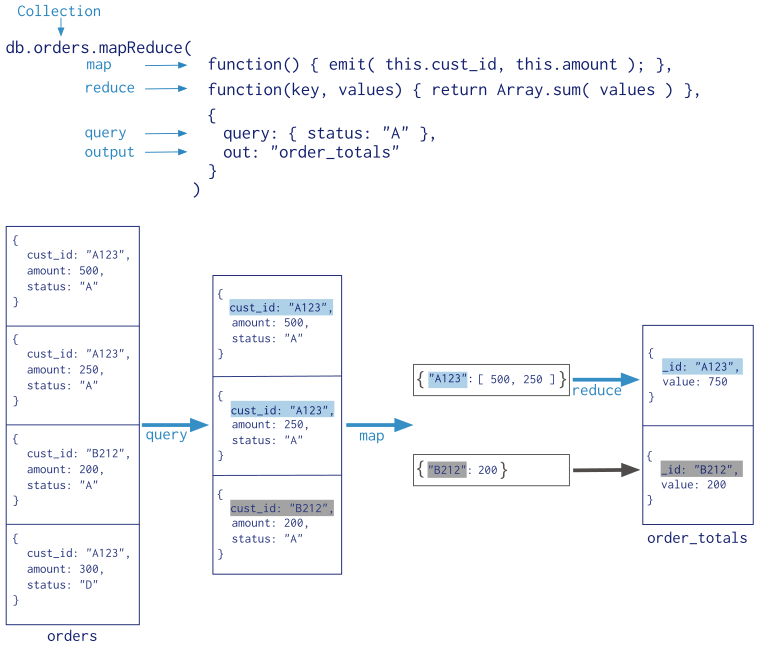
\includegraphics[width=0.8\textheight]{imgs/map-reduce.png}
  \end{center}
\end{frame}

\begin{frame}{Aggregation Operations (5): Aggregation Pipeline}
  \begin{itemize}
    \item modeled on the concept of data processing pipelines
      \inote{multi-stage pipeline as an alternative to Map-Reduce}
  \end{itemize}
  \begin{center}
    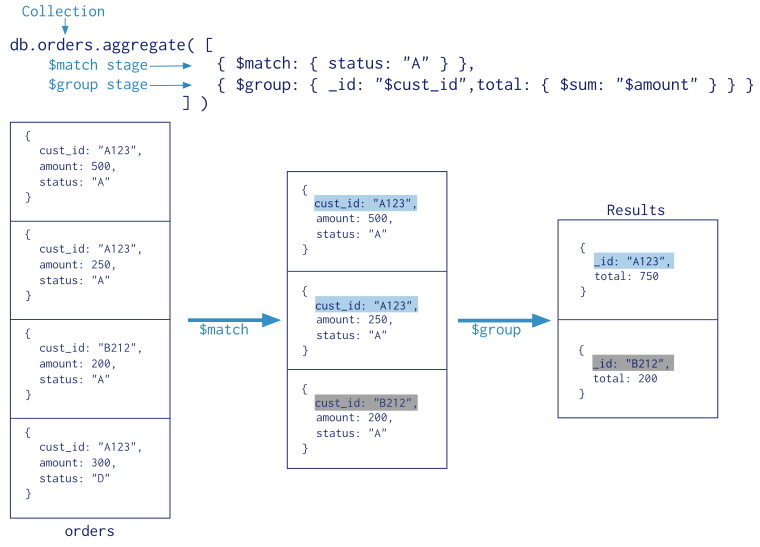
\includegraphics[width=0.8\textheight]{imgs/aggregation-pipeline.png}
  \end{center}
\end{frame}


    \begin{frame}{Advanced Write Operations (1): Atomicity}
  \begin{itemize}
      \item MongoDB write operations are atomic on the level of a document
        \inote{if two properties are update don one document nothing can happen in between}
      \item there are several so called ``write concerns''
      \begin{itemize}
        \item Guarantee that something is actually written to the database
        \item can provide different levels of guarantee
      \end{itemize}
  \end{itemize}
\end{frame}

\begin{frame}{Advanced Write Operations(2): Write concerns}
  \begin{itemize}
    \item there are four levels
    \begin{itemize}
      \item Unacknowledged
        \inote{returns immediatly}
      \item Acknowledged (default)
        \inote{write to the database then return}
      \item Journaled
        \inote{write to Journal ($=$ disk) then return}
      \item Replica Acknowledged
        \inote{write to database and backups then return}
    \end{itemize}
  \end{itemize}
\end{frame}

\begin{frame}{Advanced Write Operations (3): Transactions}
  \begin{itemize}
    \item sometimes more than a single operation needs to be atomic
      \inote{for example transfer money from one account to another}
    \item we want to ensure that either all or none of the operations are run
      \inote{we run them in one so-called transaction}
    \item MongoDB does this with so-called ``Bulk Write Operations''
      \inote{we do not go into details here}
  \end{itemize}
\end{frame}


    \begin{frame}{Conclusion (1) : Summary}
    \begin{itemize}
      \item MongoDB is a document oriented database
        \inote{Databases, Collections, Documents}
      \item Queries can be done using a javascript-style syntax
        \inote{documents are JSON}
      \item All queries \& write operations are JSON
        \inote{use javascript only for determining the operation itself}
      \item Easy to get started, supports also more complicated operations
    \end{itemize}
\end{frame}

\begin{frame}{Conclusion (2) : Further topics}
    \begin{itemize}
      \item Integration into programming languages
        \inote{perfect for JavaScript environments like node}
      \item Indexing
        \inote{be faster when searching}
      \item Mongoose: Object-oriented mapper for mongo
        \inote{when you want to have a schema}
      \item $\dots$
    \end{itemize}
\end{frame}


    \begin{frame}{The end}
      {\huge
        Thank you for your attention!\\
        Any Questions, Comments, etc?
      }

      \begin{itemize}
        \item Sources:
        \begin{itemize}
          \item \url{https://docs.mongodb.org/manual/}
          \item \url{https://en.wikipedia.org/wiki/MongoDB}
        \end{itemize}
        \item Image Sources:
        \begin{itemize}
          \item \url{https://www.mongodb.com/brand-resources}
          \item \url{https://docs.mongodb.org/manual/_images/map-reduce.png}
          \item \url{https://docs.mongodb.org/manual/_images/aggregation-pipeline.png}
        \end{itemize}
      \end{itemize}
    \end{frame}
\end{document}
